\begin{figure}[H]
    \centering
    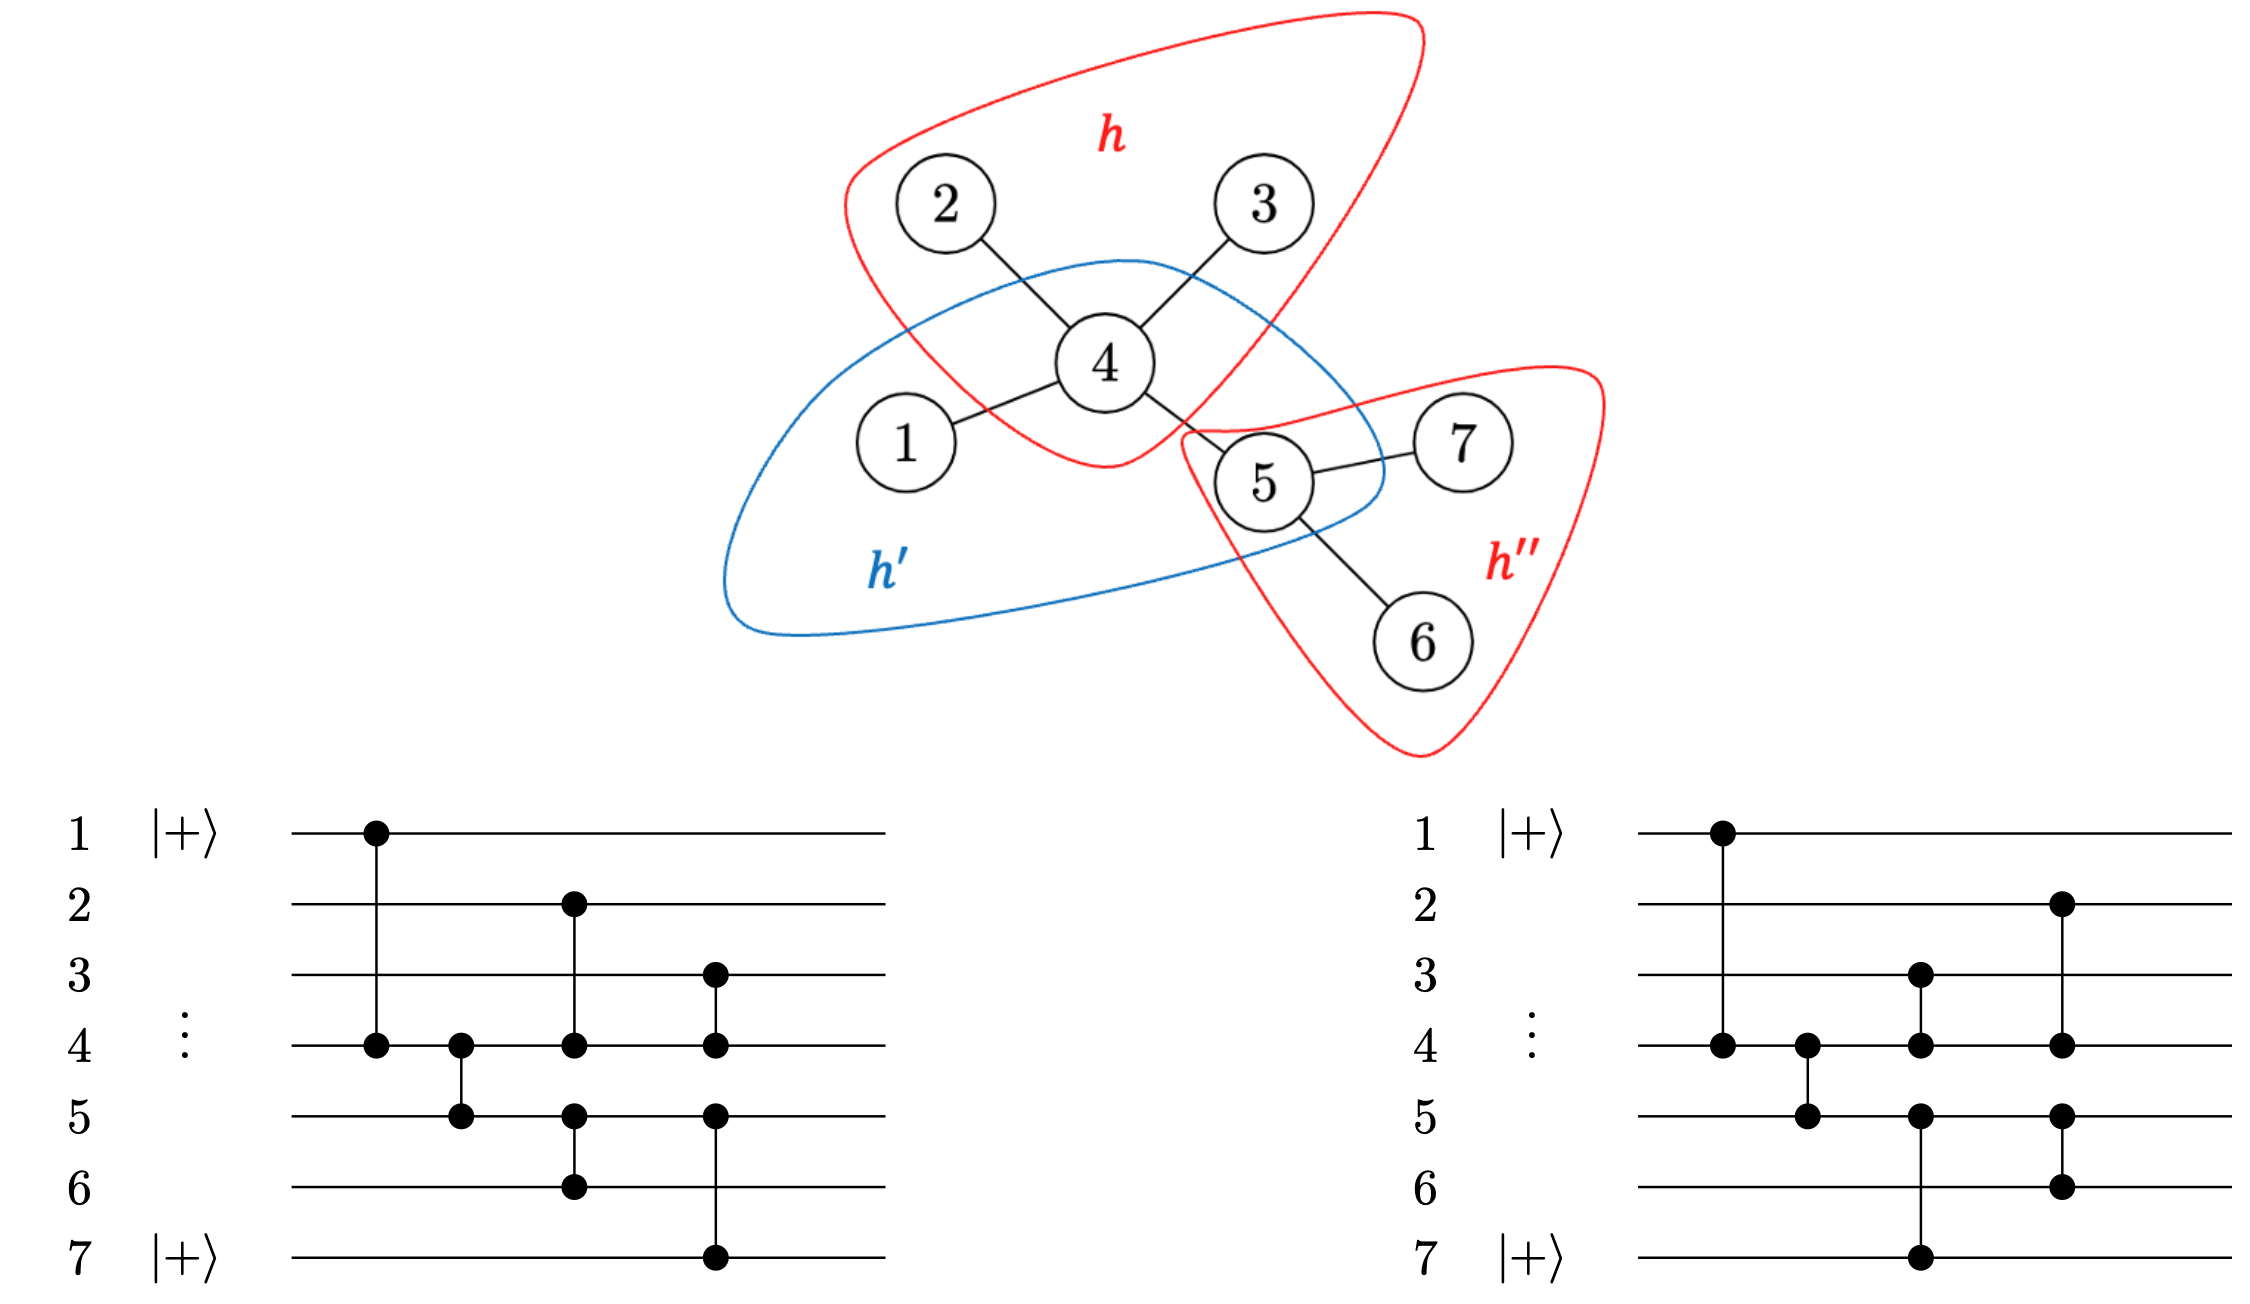
\includegraphics[scale=0.35]{singlecolor.png}
    \caption{Parallelizing the noise parameter estimation. (Top) Construction of the graph \(H\) from the edges of \(G\). An ordered triple, e.g.~\(h\), covers two adjacent edges in \(G\). These triples form the vertices \(W\) of \(H\). There is an edge in \(H\) between \(h\) and \(h'\) as they share vertices in \(G\). On the contrary \(h\) and \(h''\) are not connected by an edge in \(H\). As a consequence it is possible to fix the order of the \(\CZ\) gates corresponding to the edges covered by \(h\) and \(h''\) independently, which implies parallelization. (Left) and (Right) show how, in such situation, two orderings are enough to extract \(\lambda_{(2,4),4}, \lambda_{(3,4),4}, \lambda_{(5,6),5},  \lambda_{(5,7),5}\).}
	\label{fig:single-color-ordering}
\end{figure}
